\documentclass[a4paper,14pt]{extarticle}

\usepackage[utf8x]{inputenc}
\usepackage[T1,T2A]{fontenc}
\usepackage[russian]{babel}
\usepackage{hyperref}
\usepackage{indentfirst}
\usepackage{here}
\usepackage{array}
\usepackage{graphicx}
\usepackage{caption}
\usepackage{subcaption}
\usepackage{chngcntr}
\usepackage{amsmath}
\usepackage{amssymb}
\usepackage{amsthm}
\usepackage{pgfplots}
\usepackage{pgfplotstable}
\usepackage[left=2cm,right=2cm,top=2cm,bottom=2cm,bindingoffset=0cm]{geometry}
\usepackage{multicol}
\usepackage{askmaps}
\usepackage{titlesec}
\usepackage{listings}
\usepackage{color}
\usepackage{enumerate}
\usepackage{hhline}
\usepackage{enumitem}
\usepackage{courier}
\usepackage{wrapfig}
\usetikzlibrary{arrows,automata}

\setitemize{itemsep=0em}
\setenumerate{itemsep=0em}

\theoremstyle{definition}

\pgfkeys{/pgf/number format/.cd,1000 sep={\,}}

\definecolor{green}{rgb}{0,0.6,0}
\definecolor{gray}{rgb}{0.5,0.5,0.5}
\definecolor{purple}{rgb}{0.58,0,0.82}

\lstset{
	language=python,
	backgroundcolor=\color{white},   
	commentstyle=\color{green},
	keywordstyle=\color{blue},
	numberstyle=\tiny\color{gray},
	stringstyle=\color{purple},
	basicstyle=\footnotesize\ttfamily,
	breakatwhitespace=false,
	breaklines=true,
	captionpos=b,
	keepspaces=true,
	numbers=left,
	numbersep=5pt,
	showspaces=false,
	showstringspaces=false,
	showtabs=false,
	tabsize=2,
	frame=single,
	inputpath={../code/}
}

\renewcommand{\le}{\ensuremath{\leqslant}}
\renewcommand{\leq}{\ensuremath{\leqslant}}
\renewcommand{\ge}{\ensuremath{\geqslant}}
\renewcommand{\geq}{\ensuremath{\geqslant}}
\renewcommand{\epsilon}{\ensuremath{\varepsilon}}
\renewcommand{\phi}{\ensuremath{\varphi}}
\renewcommand{\thefigure}{\arabic{figure}} 	
\newcommand{\norm}[1]{\left\lVert#1\right\rVert}
\newcommand*\sfrac[2]{{}^{#1}\!/_{#2}}

%\titleformat*{\section}{\large\bfseries} 
\titleformat*{\subsection}{\normalsize\bfseries} 
\titleformat*{\subsubsection}{\normalsize\bfseries} 
\titleformat*{\paragraph}{\normalsize\bfseries} 
\titleformat*{\subparagraph}{\normalsize\bfseries} 

\counterwithin{figure}{section}
\counterwithin{equation}{section}
\counterwithin{table}{section}
\newcommand{\sign}[1][5cm]{\makebox[#1]{\hrulefill}}
\graphicspath{{../pics/}}
\captionsetup{justification=centering,margin=1cm}
\setlength\parindent{5ex}
\def\arraystretch{1.3}
\def\tabcolsep{12pt}
%\titlelabel{\thetitle.\quad}

\DeclareMathOperator*{\argmin}{argmin}
\DeclareMathOperator*{\argmax}{argmax}

\begin{document}

\begin{titlepage}
\begin{center}
	\textbf{Санкт-Петербургский Политехнический Университет \\Петра Великого}\\[0.3cm]
	\small Институт компьютерных наук и технологий \\[0.3cm]
	\small Кафедра компьютерных систем и программных технологий\\[4cm]
	
	\textbf{ОТЧЕТ}\\ \textbf{по расчетному заданию}\\[0.5cm]
	\textbf{<<Построение моделей>>}\\[0.1cm]
	\textbf{Системный анализ и принятие решений}\\[8.0cm]
\end{center}

\begin{flushright}
	\begin{minipage}{0.4\textwidth}
		\begin{flushleft}
			\small \textbf{Работу выполнил студент}\\[3mm]
			\small группа 33501/4 \hspace*{6mm} Дьячков В.В.\\[5mm]
			
			\small \textbf{Преподаватель}\\[5mm]
		 	\small \sign[3cm] \hspace*{5mm} Сабонис С.С.\\[0.5cm]
		\end{flushleft}
	\end{minipage}
\end{flushright}

\vfill

\begin{center}
	\small Санкт-Петербург\\
	\small \the\year
\end{center}
\end{titlepage}

\addtocounter{page}{1}

\tableofcontents
%\newpage
\listoffigures
%\listoftables
\newpage

\section{Техническое задание}

\begin{enumerate}
	\setlength{\itemsep}{0em}
	\item Записать необходимые условия оптимальности для задачи и решить задачу аналитически;
	\item Решить задачу методом релаксации;
	\item Решить задачу методом наискорейшего подъема;
	\item Решить задачу методом Ньютона;
	\item Решить задачу методом сопряженных градиентов;
	\item Решить задачу методом Бройдена.
\end{enumerate}

\section{Исходные данные}

\paragraph{Вариант 32}

Дана задача нелинейного программирования:
\begin{equation*}
	\max f(X) = \max \left( -31 x_1^2 - 34 x_2^2 + 4 x_1 x_2 + 286 x_1 + 388 x_2 \right)
\end{equation*}

\section{Аналитическое решение}

\newtheorem*{theorem1}{Необходимое условие максимума первого порядка}
\begin{theorem1}
Пусть $f(X)$ дифференцируема в точке $X^* \in R^n$. Тогда если $X^*$ -- локальный экстремум, то $f'(X^*) = 0$. 
\end{theorem1}

\newtheorem*{theorem2}{Достаточное условие максимума второго порядка}
\begin{theorem2}
Пусть $f(X)$ дважды дифференцируема в точке $X^* \in R^n$. Тогда если $f'(X^*) = 0$, матрица $H(X^*)$ отрицательно определена (полуопределена), то $X^*$ -- строгий (нестрогий) локальный экстремум.
\end{theorem2}

Вычислим частные производные 1 и 2 порядка:
\begin{multicols}{2}
	\centering
	$\dfrac{\partial f}{\partial x_1} \left(X\right) = -62 x_1 + 4 x_2 + 286$\\
	$\dfrac{\partial f}{\partial x_2} \left(X\right) = -68 x_2 + 4 x_1 + 388$
\end{multicols}

\begin{multicols}{3}
	\centering
	$\dfrac{\partial^2 f}{\partial x_1^2} \left(X\right) = -62$\\
	$\dfrac{\partial^2 f}{\partial x_1 \partial x_2} \left(X\right) = 4$\\
	$\dfrac{\partial^2 f}{\partial x_2^2} \left(X\right) = -68$
\end{multicols}
\vspace{0.3cm}

Следовательно матрица Гессе $H(X)$ равна:
\begin{equation*}
H(X) = H = 
\begin{pmatrix}
	-62 & 4 \\
	4 & -68
\end{pmatrix}
\end{equation*}\\

\newtheorem*{theorem3}{Критерий отрицательной определенности квадратичной формы}
\begin{theorem3}
Для отрицательной определенности квадратичной формы необходимо и достаточно, чтобы угловые миноры четного порядка ее матрицы были положительны, а нечетного порядка — отрицательны.
\end{theorem3}

Найдем главные миноры матрицы $H$:
\begin{multicols}{2}
\centering
$\Delta_1 = \begin{vmatrix} -62 \end{vmatrix} = -62$\\
$\Delta_2 = \begin{vmatrix}
	-62 & 4 \\
	4 & -68
\end{vmatrix} = 4200$
\end{multicols}
По критерию отрицательной определенности квадратичной формы, матрица $H$ отрицательно определена (выполнено достаточное условие максимума второго порядка).

Найдем точку $X^*$:
\begin{align*}
&\begin{cases}
	-68 x_2 + 4 x_1 + 388 = 0 \\
	-62 x_1 + 4 x_2 + 286 = 0 
\end{cases}\Rightarrow
\begin{cases}
	x_1 = 17 x_2 - 97 \\
	-62 \cdot (17 x_2 - 97) + 4 x_2 + 286 = 0
\end{cases}\Rightarrow \\
&\begin{cases}
	x_1 = 17 x_2 - 97 \\
	-1050 x_2 + 6300 = 0
\end{cases}\Rightarrow
\begin{cases}
	x_1 = 17 x_2 - 97 \\
	x_2 = 6
\end{cases}\Rightarrow
\begin{cases}
	x_1 = 5 \\
	x_2 = 6
\end{cases}
\end{align*}

Следовательно максимум функции $f(X)$ достигается в точке $X^* = (5, 6)$: $f(X^*) = 1879$.

\section{Решение методом релаксации}

\subsection{Описание метода}

Траектория поиска решения:
\begin{equation*}
X^{(i+1,j)}  = X^{(i,j)} + t^{(i)} K^{(i,j)},
\end{equation*}
где $t^{(i)}$ -- длина шага, $K^{(i)}$ -- вектор направления.

%\begin{equation*}
%t^{(i,j)} = -\left[ \dfrac{\partial^2 f}{\partial x_j^2} \left(X^{(i,j)} \right) \right]^{-1}
%\end{equation*}

\begin{equation*}
t^{(i)} = -\dfrac{\nabla^T f\left(X^{(i)}\right) K^{(i)}}{K^{(i)^T} H\left(X^{(i)}\right) K^{(i)}}
\end{equation*}

\begin{equation*}
K^{(i,j)} = \begin{bmatrix} K_1^{(i,j)} & \cdots & K_n^{(i,j)} \end{bmatrix}
\end{equation*}

\begin{equation*}
K_k^{(i,j)} = 
\begin{cases}
\dfrac{\partial f}{\partial x_j}\left( X^{(i,j)} \right), &k = j\\
0, &k \neq j
\end{cases}
\end{equation*}

%\begin{equation*}
%x_j^{(i+1,j)} = x_j^{(i,j)} - \dfrac{\partial f}{\partial x_j}\left( X^{(i,j)} \right) \cdot \left[ \dfrac{\partial^2 f}{\partial x_j^2} \left(X^{(i,j)} \right) \right]^{-1}
%\end{equation*}

%$X^{(i)} = [x^{(i,1)}, x^{(i,2)}]$
%
%$X^{i} \rightarrow X^{(i,1)} \rightarrow X^{(i,2)} = X^{i+1}$
%
%$\Delta x_j^{i+1} = x_j^{(i+1,j)} - x_j^{(i,j)}$
%
%$\Delta f\left(\Delta x_j\right) = f\left( X^{(i+1,j)}\right) - f\left( X^{(i+1,j-1)}\right)$
%
%$\Delta x_j = \argmax \limits_{(\Delta x_j)} \left\lbrace \Delta f\left(\Delta x_j\right) \right\rbrace$

\newpage

\subsection{Исходный код}

\lstinputlisting[caption=relaxation.py, label=code:1]{relaxation.py}

\subsection{Траектории поиска}

Выберем 4 начальные точки разной степени удаленности от оптимальной ($x_1 = 5, x_2 = 6$): 
\begin{multicols}{2} 
\begin{enumerate}
	\setlength{\itemsep}{0em}
	\item $x_1 = 0, x_2 = 0$
	\item $x_1 = 1, x_2 = 8$
	\item $x_1 = 6, x_2 = 5$
	\item $x_1 = 10, x_2 = 10$
\end{enumerate}
\end{multicols}

\begin{table}[H]
\begin{center}
	\pgfkeys{/pgf/number format/.cd,1000 sep={\,}}
	\begin{multicols}{2}
	\pgfplotstabletypeset[col sep=comma,
	    columns={x1, x2, f},
	    column type/.add={|c|}{},
	    columns/r/.style={column name={Код}},
	    columns/x1/.style={fixed, precision=3, zerofill, column name={$x_1$}},
	    columns/x2/.style={fixed, precision=3, zerofill, column name={$x_2$}},
	    columns/f/.style={fixed, precision=3, zerofill, column name={$f(X)$}},
	    every nth row={1}{before row=\hline},
	    every head row/.style={before row=\hline, after row=\hline, },
	    every last row/.style={after row=\hline}
	   ]{../data/relaxation_1.csv}
	   \caption{$X = (0, 0)$}
	   \vspace{0.5cm}
	\pgfplotstabletypeset[col sep=comma,
	    columns={x1, x2, f},
	    column type/.add={|c|}{},
	    columns/r/.style={column name={Код}},
	    columns/x1/.style={fixed, precision=3, zerofill, column name={$x_1$}},
	    columns/x2/.style={fixed, precision=3, zerofill, column name={$x_2$}},
	    columns/f/.style={fixed, precision=3, zerofill, column name={$f(X)$}},
	    every nth row={1}{before row=\hline},
	    every head row/.style={before row=\hline, after row=\hline, },
	    every last row/.style={after row=\hline}
	   ]{../data/relaxation_2.csv}
	   \caption{$X = (1, 8)$}
	   \vspace{0.5cm}
	\end{multicols}
\end{center}
\end{table}
\vspace{-1cm}
\begin{table}[H]
\begin{center}
	\begin{multicols}{2}
	\pgfplotstabletypeset[col sep=comma,
	    columns={x1, x2, f},
	    column type/.add={|c|}{},
	    columns/r/.style={column name={Код}},
	    columns/x1/.style={fixed, precision=3, zerofill, column name={$x_1$}},
	    columns/x2/.style={fixed, precision=3, zerofill, column name={$x_2$}},
	    columns/f/.style={fixed, precision=3, zerofill, column name={$f(X)$}},
	    every nth row={1}{before row=\hline},
	    every head row/.style={before row=\hline, after row=\hline, },
	    every last row/.style={after row=\hline}
	   ]{../data/relaxation_3.csv}
	   \caption{$X = (6, 5)$}
	   \vspace{0.5cm}
	\pgfplotstabletypeset[col sep=comma,
	    columns={x1, x2, f},
	    column type/.add={|c|}{},
	    columns/r/.style={column name={Код}},
	    columns/x1/.style={fixed, precision=3, zerofill, column name={$x_1$}},
	    columns/x2/.style={fixed, precision=3, zerofill, column name={$x_2$}},
	    columns/f/.style={fixed, precision=3, zerofill, column name={$f(X)$}},
	    every nth row={1}{before row=\hline},
	    every head row/.style={before row=\hline, after row=\hline, },
	    every last row/.style={after row=\hline}
	   ]{../data/relaxation_4.csv}
	   \caption{$X = (10, 10)$}
	   \vspace{0.5cm}
	\end{multicols}
\end{center}
\end{table}

На рис. \ref{fig:relaxation} изображены траектории поиска точки максимума $X = (5, 6)$ методом релаксации при разных начальных точках.
\begin{figure}[H]
\begin{center}
	\begin{subfigure}[b]{0.49\textwidth}
		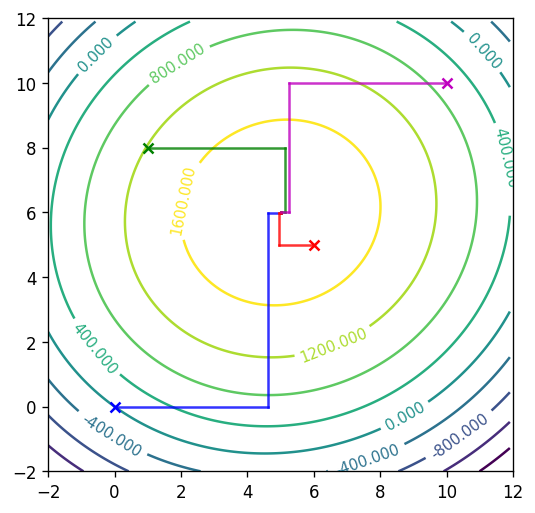
\includegraphics[width=0.96\textwidth]{relaxation}
	\end{subfigure}
	\begin{subfigure}[b]{0.49\textwidth}
		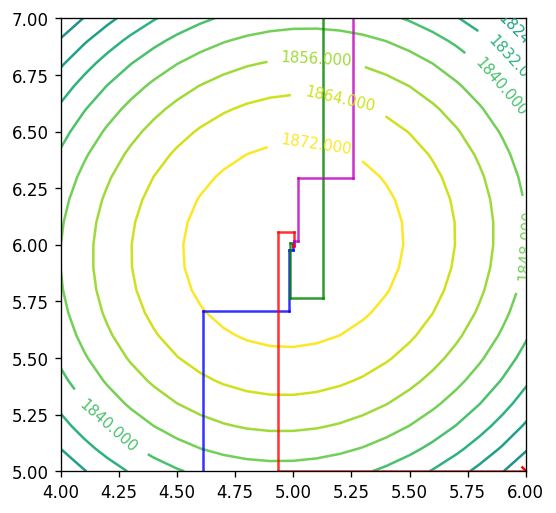
\includegraphics[width=\textwidth]{relaxation_zoom}
	\end{subfigure}
	\caption{Траектории поиска методом релаксации}
	\label{fig:relaxation}
\end{center}
\end{figure}

\section{Решение методом наискорейшего подъема}

\subsection{Описание метода}

Траектория поиска решения:
\begin{equation*}
X^{(i+1)}  = X^{(i)} + t^{(i)} K^{(i)},
\end{equation*}
где $t^{(i)}$ -- длина шага, $K^{(i)}$ -- вектор направления.

\begin{equation*}
t^{(i)} = -\dfrac{\nabla^T f\left(X^{(i)}\right) K^{(i)}}{K^{(i)^T} H\left(X^{(i)}\right) K^{(i)}}
\end{equation*}

\begin{equation*}
K^{(i)} = \nabla f(X)
\end{equation*}

%Линейная аппроксимация целевой функции в точке $X^{(i)}$:
%
%\begin{align*}
%f\left(X^{(i+1)}\right) &\approx f\left(X^{(i)}\right) + \left\langle f'(X^{(i)}), X^{(i+1)} - X^{(i)} \right\rangle \\ 
%&= f\left(X^{(i)}\right) + f'\left(X^{(i)}\right)^T \left(X^{(i+1)} - X^{(i)}\right)
%\end{align*}
%
%$X^{(i+1)} = X^{(i)} + t^{(i)} K^{(i)}$
%
%$\Delta f = f\left(X^{(i+1)}\right) - f\left(X^{(i)}\right) = 
%t^{(i)} \left\langle f'(X^{(i)}), X^{(i+1)} - X^{(i)} \right\rangle$
%
%$t^{(i)} = \argmax \limits_{(K^{(i)})} \left\lbrace \sum\limits_{k=1}^n \dfrac{\partial f}{\partial x_k} \left( X^{(i)} \right) K_k^{(i)} \right\rbrace$ при условии $\sum\limits_{k=1}^n \left[ K_k^{(i)} \right]^2 = 1$.
%
%\begin{equation*}
%K_k^{(i)} = \frac{\dfrac{\partial f}{\partial x_k} \left(X^{(i)}\right)}{\sqrt{\sum\limits_{k=1}^n \left[ \dfrac{\partial f}{\partial x_k} \left(X^{(i)}\right) \right]^2}} \Longleftrightarrow
%K_k^{(i)} = \frac{f'\left(X^{(i)}\right)}{\norm{f'\left(X^{(i)}\right)}}
%\end{equation*}

\subsection{Исходный код}

\lstinputlisting[caption=steepest\_ascent.py, label=code:1]{steepest_ascent.py}

\subsection{Траектории поиска}

Выберем 4 начальные точки разной степени удаленности от оптимальной ($x_1 = 5, x_2 = 6$):
\begin{multicols}{2} 
\begin{enumerate}
	\setlength{\itemsep}{0em}
	\item $x_1 = 0, x_2 = 0$
	\item $x_1 = 1, x_2 = 8$
	\item $x_1 = 6, x_2 = 5$
	\item $x_1 = 10, x_2 = 10$
\end{enumerate}
\end{multicols}

\vspace{-0.5cm}
\begin{table}[H]
\begin{center}
	\begin{multicols}{2}
	\pgfplotstabletypeset[col sep=comma,
	    columns={x1, x2, f},
	    column type/.add={|c|}{},
	    columns/r/.style={column name={Код}},
	    columns/x1/.style={fixed, precision=3, zerofill, column name={$x_1$}},
	    columns/x2/.style={fixed, precision=3, zerofill, column name={$x_2$}},
	    columns/f/.style={fixed, precision=3, zerofill, column name={$f(X)$}},
	    every nth row={1}{before row=\hline},
	    every head row/.style={before row=\hline, after row=\hline, },
	    every last row/.style={after row=\hline}
	   ]{../data/steepest_ascent_1.csv}
	   \caption{$X = (0, 0)$}
	   \vspace{0.5cm}
	\pgfplotstabletypeset[col sep=comma,
	    columns={x1, x2, f},
	    column type/.add={|c|}{},
	    columns/r/.style={column name={Код}},
	    columns/x1/.style={fixed, precision=3, zerofill, column name={$x_1$}},
	    columns/x2/.style={fixed, precision=3, zerofill, column name={$x_2$}},
	    columns/f/.style={fixed, precision=3, zerofill, column name={$f(X)$}},
	    every nth row={1}{before row=\hline},
	    every head row/.style={before row=\hline, after row=\hline, },
	    every last row/.style={after row=\hline}
	   ]{../data/steepest_ascent_2.csv}
	   \caption{$X = (1, 8)$}
	   \vspace{0.5cm} 
	\end{multicols} 
\end{center}
\end{table}
\vspace{-1cm}
\begin{table}[H]
\begin{center}
	\begin{multicols}{2}
	\pgfplotstabletypeset[col sep=comma,
	    columns={x1, x2, f},
	    column type/.add={|c|}{},
	    columns/r/.style={column name={Код}},
	    columns/x1/.style={fixed, precision=3, zerofill, column name={$x_1$}},
	    columns/x2/.style={fixed, precision=3, zerofill, column name={$x_2$}},
	    columns/f/.style={fixed, precision=3, zerofill, column name={$f(X)$}},
	    every nth row={1}{before row=\hline},
	    every head row/.style={before row=\hline, after row=\hline, },
	    every last row/.style={after row=\hline}
	   ]{../data/steepest_ascent_3.csv}
	   \caption{$X = (6, 5)$}
	   \vspace{0.5cm}
	\pgfplotstabletypeset[col sep=comma,
	    columns={x1, x2, f},
	    column type/.add={|c|}{},
	    columns/r/.style={column name={Код}},
	    columns/x1/.style={fixed, precision=3, zerofill, column name={$x_1$}},
	    columns/x2/.style={fixed, precision=3, zerofill, column name={$x_2$}},
	    columns/f/.style={fixed, precision=3, zerofill, column name={$f(X)$}},
	    every nth row={1}{before row=\hline},
	    every head row/.style={before row=\hline, after row=\hline, },
	    every last row/.style={after row=\hline}
	   ]{../data/steepest_ascent_4.csv}
	   \caption{$X = (10, 10)$}
	   \vspace{0.5cm}
	\end{multicols}
\end{center}
\end{table}
\vspace{-0.5cm}

На рис. \ref{fig:steepest_ascent} изображены траектории поиска точки максимума $X = (5, 6)$ методом наискорейшего подъема при разных начальных точках.
\vspace{-0.5cm}
\begin{figure}[H]
\begin{center}
	\begin{subfigure}[b]{0.49\textwidth}
		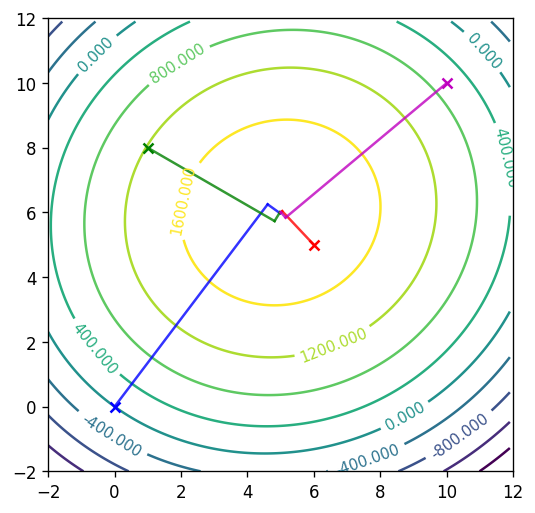
\includegraphics[width=0.96\textwidth]{steepest_ascent}
	\end{subfigure}
	\begin{subfigure}[b]{0.49\textwidth}
		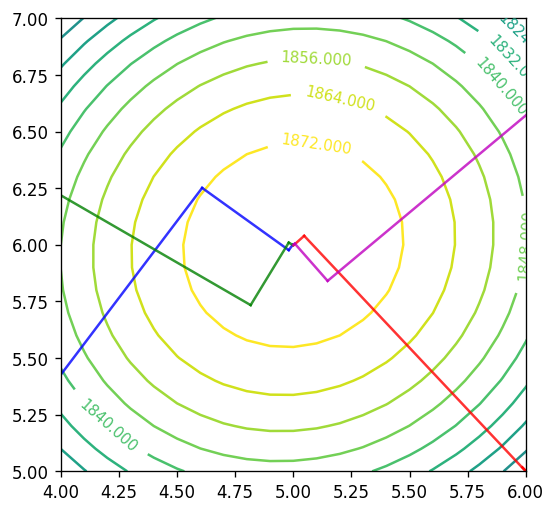
\includegraphics[width=\textwidth]{steepest_ascent_zoom}
	\end{subfigure}
	\caption{Траектории поиска методом наискорейшего подъема}
	\label{fig:steepest_ascent}
\end{center}
\end{figure}

\section{Решение методом Ньютона}

\subsection{Описание метода}

Траектория поиска решения:
\begin{equation*}
X^{(i+1)}  = X^{(i)} + t^{(i)} K^{(i)},
\end{equation*}
где $t^{(i)}$ -- длина шага, $K^{(i)}$ -- вектор направления.

\begin{equation*}
t^{(i)} = t \equiv 1
\end{equation*}

\begin{equation*}
K^{(i)} = -H^{-1}\left(X^{(i)}\right) \nabla f(X)
\end{equation*}

Для квадратичных функций метод Ньютона сходится за 1 шаг.

\subsection{Исходный код}

\lstinputlisting[caption=newton.py, label=code:1]{newton.py}

\subsection{Траектории поиска}

Выберем 4 начальные точки разной степени удаленности от оптимальной ($x_1 = 5, x_2 = 6$): 
\begin{multicols}{2} 
\begin{enumerate}
	\setlength{\itemsep}{0em}
	\item $x_1 = 0, x_2 = 0$
	\item $x_1 = 1, x_2 = 8$
	\item $x_1 = 6, x_2 = 5$
	\item $x_1 = 10, x_2 = 10$
\end{enumerate}
\end{multicols}

\begin{table}[H]
\begin{center}
	\begin{multicols}{2}
	\pgfplotstabletypeset[col sep=comma,
	    columns={x1, x2, f},
	    column type/.add={|c|}{},
	    columns/r/.style={column name={Код}},
	    columns/x1/.style={fixed, precision=3, zerofill, column name={$x_1$}},
	    columns/x2/.style={fixed, precision=3, zerofill, column name={$x_2$}},
	    columns/f/.style={fixed, precision=3, zerofill, column name={$f(X)$}},
	    every nth row={1}{before row=\hline},
	    every head row/.style={before row=\hline, after row=\hline, },
	    every last row/.style={after row=\hline}
	   ]{../data/newton_1.csv}
	   \caption{$X = (0, 0)$}
	   \vspace{0.5cm}
	\pgfplotstabletypeset[col sep=comma,
	    columns={x1, x2, f},
	    column type/.add={|c|}{},
	    columns/r/.style={column name={Код}},
	    columns/x1/.style={fixed, precision=3, zerofill, column name={$x_1$}},
	    columns/x2/.style={fixed, precision=3, zerofill, column name={$x_2$}},
	    columns/f/.style={fixed, precision=3, zerofill, column name={$f(X)$}},
	    every nth row={1}{before row=\hline},
	    every head row/.style={before row=\hline, after row=\hline, },
	    every last row/.style={after row=\hline}
	   ]{../data/newton_2.csv}
	   \caption{$X = (1, 8)$}
	   \vspace{0.5cm} 
	\end{multicols}
\end{center}
\end{table}
\vspace{-1cm}
\begin{table}[H]
\begin{center} 
	\begin{multicols}{2}
	\pgfplotstabletypeset[col sep=comma,
	    columns={x1, x2, f},
	    column type/.add={|c|}{},
	    columns/r/.style={column name={Код}},
	    columns/x1/.style={fixed, precision=3, zerofill, column name={$x_1$}},
	    columns/x2/.style={fixed, precision=3, zerofill, column name={$x_2$}},
	    columns/f/.style={fixed, precision=3, zerofill, column name={$f(X)$}},
	    every nth row={1}{before row=\hline},
	    every head row/.style={before row=\hline, after row=\hline, },
	    every last row/.style={after row=\hline}
	   ]{../data/newton_3.csv}
	   \caption{$X = (6, 5)$}
	   \vspace{0.5cm}
	\pgfplotstabletypeset[col sep=comma,
	    columns={x1, x2, f},
	    column type/.add={|c|}{},
	    columns/r/.style={column name={Код}},
	    columns/x1/.style={fixed, precision=3, zerofill, column name={$x_1$}},
	    columns/x2/.style={fixed, precision=3, zerofill, column name={$x_2$}},
	    columns/f/.style={fixed, precision=3, zerofill, column name={$f(X)$}},
	    every nth row={1}{before row=\hline},
	    every head row/.style={before row=\hline, after row=\hline, },
	    every last row/.style={after row=\hline}
	   ]{../data/newton_4.csv}
	   \caption{$X = (10, 10)$}
	   \vspace{0.5cm}
	\end{multicols}
\end{center}
\end{table}

На рис. \ref{fig:newton} изображены траектории поиска точки максимума $X = (5, 6)$ методом Ньютона при разных начальных точках.
\begin{figure}[H]
\begin{center}
	\begin{subfigure}[b]{0.49\textwidth}
		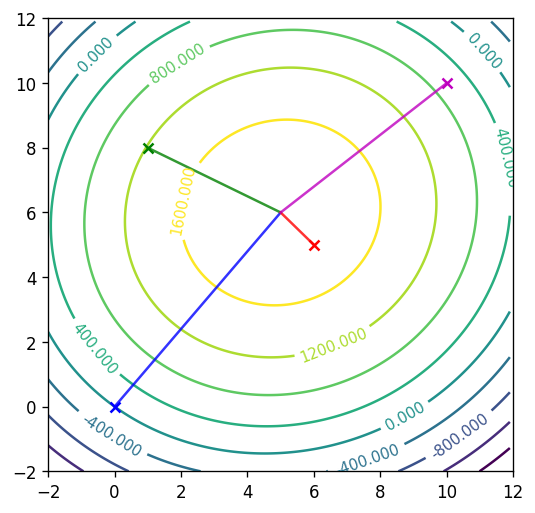
\includegraphics[width=0.96\textwidth]{newton}
	\end{subfigure}
	\begin{subfigure}[b]{0.49\textwidth}
		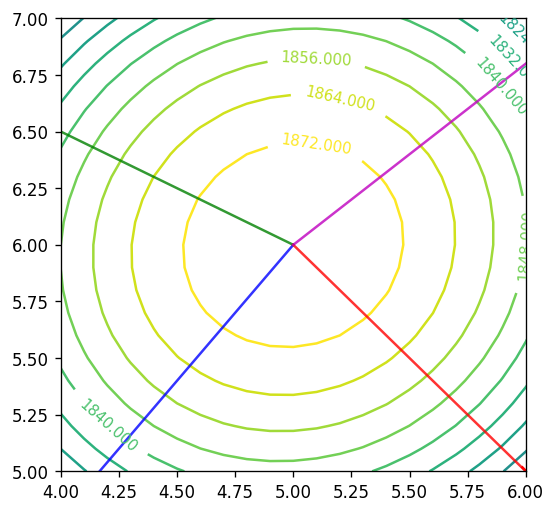
\includegraphics[width=\textwidth]{newton_zoom}
	\end{subfigure}
	\caption{Траектории поиска методом Ньютона}
	\label{fig:newton}
\end{center}
\end{figure}

\section{Решение методом сопряженных градиентов}

\subsection{Описание метода}

Траектория поиска решения:
\begin{equation*}
X^{(i+1)}  = X^{(i)} + t^{(i)} K^{(i)},
\end{equation*}
где $t^{(i)}$ -- длина шага, $K^{(i)}$ -- вектор направления.

\begin{equation*}
t^{(i)} = -\dfrac{\nabla^T f\left(X^{(i)}\right) K^{(i)}}{K^{(i)^T} H\left(X^{(i)}\right) K^{(i)}}
\end{equation*}

\begin{equation*}
K^{(i)} = 
\begin{cases}
\nabla f\left(X^{(i)}\right), &i = 0\\
\nabla f\left(X^{(i)}\right) + \dfrac{\norm{\nabla f\left(X^{(i)}\right)}^2}{\norm{\nabla f\left(X^{(i-1)}\right)}^2} \nabla f\left(X^{(i-1)}\right), &i \neq 0
\end{cases}
\end{equation*}

Для квадратичных функций число шагов равно числу переменных.

\subsection{Исходный код}

\lstinputlisting[caption=conjugate\_gradients.py, label=code:1]{conjugate_gradients.py}

\subsection{Траектории поиска}

Выберем 4 начальные точки разной степени удаленности от оптимальной ($x_1 = 5, x_2 = 6$): 
\begin{multicols}{2} 
\begin{enumerate}
	\setlength{\itemsep}{0em}
	\item $x_1 = 0, x_2 = 0$
	\item $x_1 = 1, x_2 = 8$
	\item $x_1 = 6, x_2 = 5$
	\item $x_1 = 10, x_2 = 10$
\end{enumerate}
\end{multicols}

\vspace{-0.5cm}

\begin{table}[H]
\begin{center}
	\begin{multicols}{2}
	\pgfplotstabletypeset[col sep=comma,
	    columns={x1, x2, f},
	    column type/.add={|c|}{},
	    columns/r/.style={column name={Код}},
	    columns/x1/.style={fixed, precision=3, zerofill, column name={$x_1$}},
	    columns/x2/.style={fixed, precision=3, zerofill, column name={$x_2$}},
	    columns/f/.style={fixed, precision=3, zerofill, column name={$f(X)$}},
	    every nth row={1}{before row=\hline},
	    every head row/.style={before row=\hline, after row=\hline, },
	    every last row/.style={after row=\hline}
	   ]{../data/conjugate_gradients_1.csv}
	   \caption{$X = (0, 0)$}
	   \vspace{0.5cm}
	\pgfplotstabletypeset[col sep=comma,
	    columns={x1, x2, f},
	    column type/.add={|c|}{},
	    columns/r/.style={column name={Код}},
	    columns/x1/.style={fixed, precision=3, zerofill, column name={$x_1$}},
	    columns/x2/.style={fixed, precision=3, zerofill, column name={$x_2$}},
	    columns/f/.style={fixed, precision=3, zerofill, column name={$f(X)$}},
	    every nth row={1}{before row=\hline},
	    every head row/.style={before row=\hline, after row=\hline, },
	    every last row/.style={after row=\hline}
	   ]{../data/conjugate_gradients_2.csv}
	   \caption{$X = (1, 8)$}
	   \vspace{0.5cm} 
	\end{multicols}
\end{center}
\end{table}
\vspace{-1cm}
\begin{table}[H]
\begin{center}
	\begin{multicols}{2}
	\pgfplotstabletypeset[col sep=comma,
	    columns={x1, x2, f},
	    column type/.add={|c|}{},
	    columns/r/.style={column name={Код}},
	    columns/x1/.style={fixed, precision=3, zerofill, column name={$x_1$}},
	    columns/x2/.style={fixed, precision=3, zerofill, column name={$x_2$}},
	    columns/f/.style={fixed, precision=3, zerofill, column name={$f(X)$}},
	    every nth row={1}{before row=\hline},
	    every head row/.style={before row=\hline, after row=\hline, },
	    every last row/.style={after row=\hline}
	   ]{../data/conjugate_gradients_3.csv}
	   \caption{$X = (6, 5)$}
	   \vspace{0.5cm}
	\pgfplotstabletypeset[col sep=comma,
	    columns={x1, x2, f},
	    column type/.add={|c|}{},
	    columns/r/.style={column name={Код}},
	    columns/x1/.style={fixed, precision=3, zerofill, column name={$x_1$}},
	    columns/x2/.style={fixed, precision=3, zerofill, column name={$x_2$}},
	    columns/f/.style={fixed, precision=3, zerofill, column name={$f(X)$}},
	    every nth row={1}{before row=\hline},
	    every head row/.style={before row=\hline, after row=\hline, },
	    every last row/.style={after row=\hline}
	   ]{../data/conjugate_gradients_4.csv}
	   \caption{$X = (10, 10)$}
	   \vspace{0.5cm}
	\end{multicols}
\end{center}
\end{table}
\vspace{-0.5cm}

На рис. \ref{fig:conjugate_gradient} изображены траектории поиска точки максимума $X = (5, 6)$ методом сопряженных градиентов при разных начальных точках.
\begin{figure}[H]
\begin{center}
	\begin{subfigure}[b]{0.49\textwidth}
		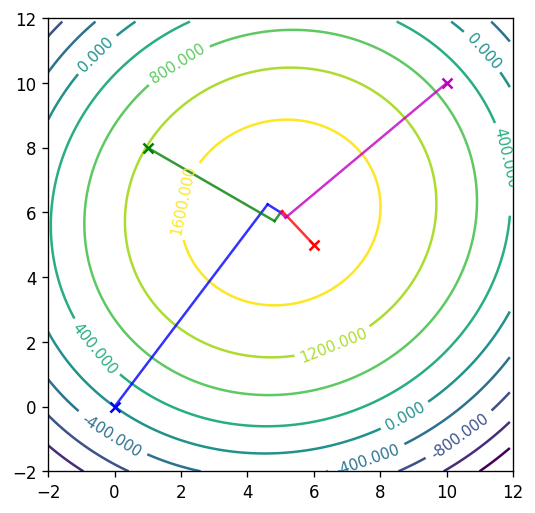
\includegraphics[width=0.96\textwidth]{conjugate_gradients}
	\end{subfigure}
	\begin{subfigure}[b]{0.49\textwidth}
		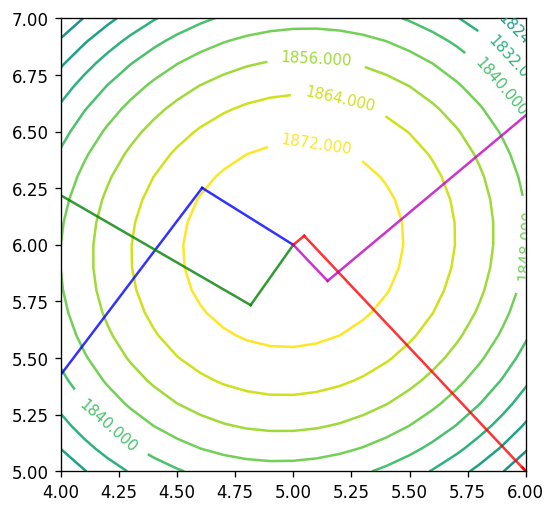
\includegraphics[width=\textwidth]{conjugate_gradients_zoom}
	\end{subfigure}
	\caption{Траектории поиска методом сопряженных градиентов}
	\label{fig:conjugate_gradient}
\end{center}
\end{figure}

\section{Решение методом Бройдена}

\subsection{Описание метода}

Траектория поиска решения:
\begin{equation*}
X^{(i+1)}  = X^{(i)} + t^{(i)} K^{(i)},
\end{equation*}
где $t^{(i)}$ -- длина шага, $K^{(i)}$ -- вектор направления.

\begin{equation*}
t^{(i)} = -\dfrac{\nabla^T f\left(X^{(i)}\right) K^{(i)}}{K^{(i)^T} H\left(X^{(i)}\right) K^{(i)}}
\end{equation*}

\begin{equation*}
K^{(i)} = -\eta^{(i)} \nabla f\left(X^{(i)}\right)
\end{equation*}

\begin{equation*}
\eta^{(i)} = 
\begin{cases}
-E, &i = 0\\
\eta^{(i-1)} + \Delta \eta^{(i-1)}, &i \neq 0
\end{cases}
\end{equation*}

\begin{equation*}
\Delta \eta^{(i-1)} = \dfrac{z^{(i-1)} \left(z^{(i-1)}\right)^T}{\left(z^{(i-1)}\right)^T \Delta g^{(i-1)}}
\end{equation*}

\begin{equation*}
z^{(i-1)} = X^{(i)} - X^{(i-1)} - \eta^{(i-1)} \Delta g^{(i-1)}
\end{equation*}

\begin{equation*}
\Delta g^{(i-1)} = \nabla f\left(X^{(i)}\right) - \nabla f\left(X^{(i-1)}\right)
\end{equation*}

\subsection{Исходный код}

\lstinputlisting[caption=broyden.py, label=code:1]{broyden.py}

\subsection{Траектории поиска}

Выберем 4 начальные точки разной степени удаленности от оптимальной ($x_1 = 5, x_2 = 6$): 
\begin{multicols}{2} 
\begin{enumerate}
	\setlength{\itemsep}{0em}
	\item $x_1 = 0, x_2 = 0$
	\item $x_1 = 1, x_2 = 8$
	\item $x_1 = 6, x_2 = 5$
	\item $x_1 = 10, x_2 = 10$
\end{enumerate}
\end{multicols}

\begin{table}[H]
\begin{center}
	\begin{multicols}{2}
	\pgfplotstabletypeset[col sep=comma,
	    columns={x1, x2, f},
	    column type/.add={|c|}{},
	    columns/r/.style={column name={Код}},
	    columns/x1/.style={fixed, precision=3, zerofill, column name={$x_1$}},
	    columns/x2/.style={fixed, precision=3, zerofill, column name={$x_2$}},
	    columns/f/.style={fixed, precision=3, zerofill, column name={$f(X)$}},
	    every nth row={1}{before row=\hline},
	    every head row/.style={before row=\hline, after row=\hline, },
	    every last row/.style={after row=\hline}
	   ]{../data/broyden_1.csv}
	   \caption{$X = (0, 0)$}
	   \vspace{0.5cm}
	\pgfplotstabletypeset[col sep=comma,
	    columns={x1, x2, f},
	    column type/.add={|c|}{},
	    columns/r/.style={column name={Код}},
	    columns/x1/.style={fixed, precision=3, zerofill, column name={$x_1$}},
	    columns/x2/.style={fixed, precision=3, zerofill, column name={$x_2$}},
	    columns/f/.style={fixed, precision=3, zerofill, column name={$f(X)$}},
	    every nth row={1}{before row=\hline},
	    every head row/.style={before row=\hline, after row=\hline, },
	    every last row/.style={after row=\hline}
	   ]{../data/broyden_2.csv}
	   \caption{$X = (1, 8)$}
	   \vspace{0.5cm} 
	\end{multicols}
\end{center}
\end{table}
\vspace{-1cm}
\begin{table}[H]
\begin{center}
	\begin{multicols}{2}
	\pgfplotstabletypeset[col sep=comma,
	    columns={x1, x2, f},
	    column type/.add={|c|}{},
	    columns/r/.style={column name={Код}},
	    columns/x1/.style={fixed, precision=3, zerofill, column name={$x_1$}},
	    columns/x2/.style={fixed, precision=3, zerofill, column name={$x_2$}},
	    columns/f/.style={fixed, precision=3, zerofill, column name={$f(X)$}},
	    every nth row={1}{before row=\hline},
	    every head row/.style={before row=\hline, after row=\hline, },
	    every last row/.style={after row=\hline}
	   ]{../data/broyden_3.csv}
	   \caption{$X = (6, 5)$}
	   \vspace{0.5cm}
	\pgfplotstabletypeset[col sep=comma,
	    columns={x1, x2, f},
	    column type/.add={|c|}{},
	    columns/r/.style={column name={Код}},
	    columns/x1/.style={fixed, precision=3, zerofill, column name={$x_1$}},
	    columns/x2/.style={fixed, precision=3, zerofill, column name={$x_2$}},
	    columns/f/.style={fixed, precision=3, zerofill, column name={$f(X)$}},
	    every nth row={1}{before row=\hline},
	    every head row/.style={before row=\hline, after row=\hline, },
	    every last row/.style={after row=\hline}
	   ]{../data/broyden_4.csv}
	   \caption{$X = (10, 10)$}
	   \vspace{0.5cm}
	\end{multicols}
\end{center}
\end{table}

На рис. \ref{fig:broyden} изображены траектории поиска точки максимума $X = (5, 6)$ методом Бройдена при разных начальных точках.
\begin{figure}[H]
\begin{center}
	\begin{subfigure}[b]{0.49\textwidth}
		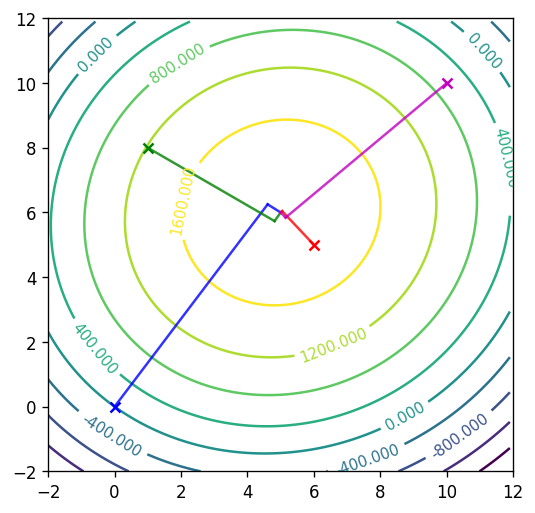
\includegraphics[width=0.96\textwidth]{broyden}
	\end{subfigure}
	\begin{subfigure}[b]{0.49\textwidth}
		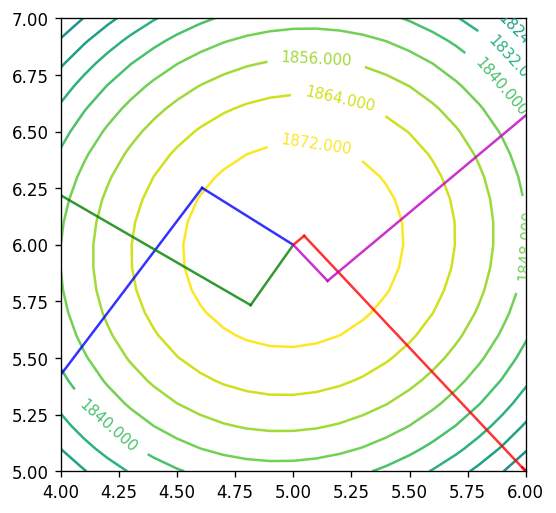
\includegraphics[width=\textwidth]{broyden_zoom}
	\end{subfigure}
	\caption{Траектории поиска методом Бройдена}
	\label{fig:broyden}
\end{center}
\end{figure}

\end{document}